	
\subsubsection{03.11.14}

\begin{enumerate}
	\item The time of beginning and ending of the meeting:
	14:00 – 21:40
	\item Purposes of the meeting:
	\begin{enumerate}
	  \item	To finish the MEL.
	  
	  \item To install the drivers for MEL.
	  
	  \item To	write a program to control MEL.
	  
	  \item To fix the the belt with threads.
	  
    \end{enumerate}
    
	\item Work that has been done:
	\begin{enumerate}
	  \item	Driver has been installed on the robot.
      
      \item	Actuators have been interconnected by a shaft which reels the belt.
      
      \item	The belt was firmly sewn to the last axle and to the shaft of MEL.
      
      \begin{figure}[H]
      	\begin{minipage}[h]{0.4\linewidth}
      		\center{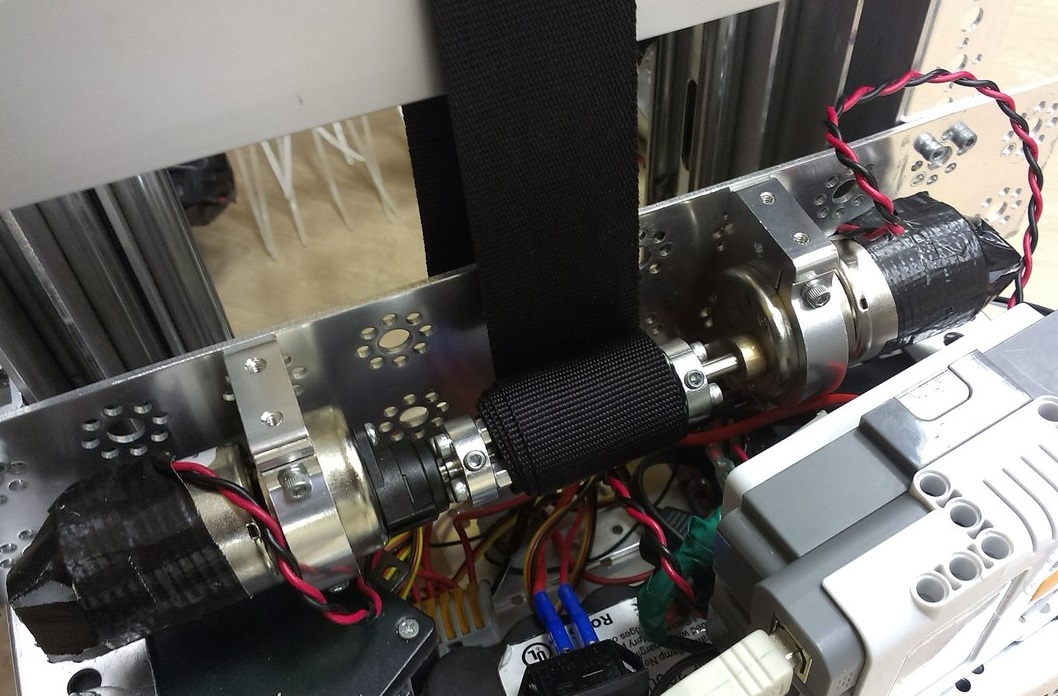
\includegraphics[scale=0.2]{days/03.11.14/images/01}}
      	\end{minipage}
      	\hfill
      	\begin{minipage}[h]{0.27\linewidth}
      		\center{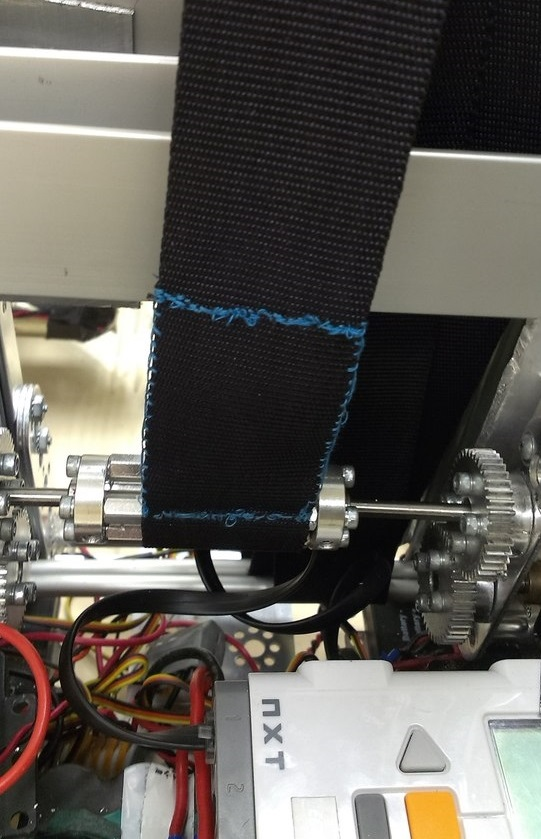
\includegraphics[scale=0.2]{days/03.11.14/images/02}}
      	\end{minipage}
      	\hfill
      	\begin{minipage}[h]{0.27\linewidth}
      		\center{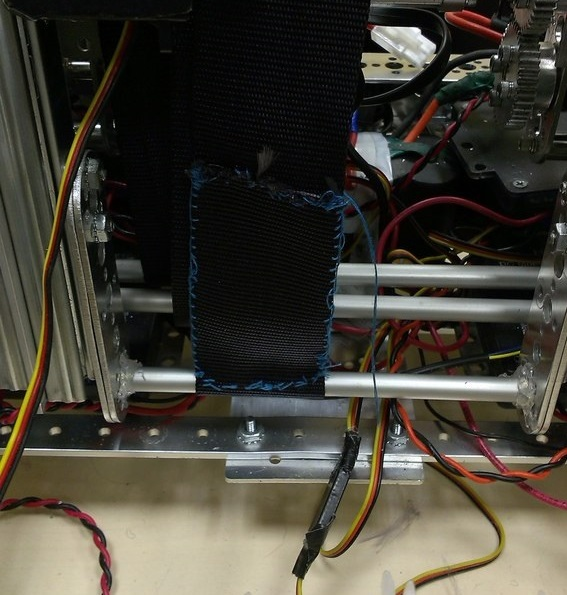
\includegraphics[scale=0.25]{days/03.11.14/images/03}}
      	\end{minipage}
      	\vfill
      	\begin{minipage}[h]{0.4\linewidth}
      		\caption{Lift}
      	\end{minipage}
      	\hfill
      	\begin{minipage}[h]{0.58\linewidth}
      		\caption{Belt was fixed}
      	\end{minipage}
      \end{figure}
      
      \item	Wrote a simple programm that can rotate the MEL with a maximum speed in each direction or stand still. The movement of the MEL is monitored by the right analog sensor.
      
      \item	It has been found that the drive shafts are not arranged coaxially, so the construction staggered. It was decided to change the design of the MEL so that the spool would be located on a separate axe. Motors will be connected to spool by the gears with a gear ratio of 1: 1. This will eliminate the problems with non-coaxial arrangement of motors.
      
    \end{enumerate}
    
	\item Results: 
	\begin{enumerate}
	  \item	The drivers have been installed on the robot.
	  
	  \item	Belt is securely fastened to the MEL.
	  
	  \item	MEL has been tested. Two drives have enough power to widen the lift.
	  
    \end{enumerate}
    
	\item Tasks for the next meetings:
	\begin{enumerate}
	  \item To alter the design of the MEL so that it will be reliable.
	  
	  \item To connect the encoder to one of the drives.
	  
    \end{enumerate}     
\end{enumerate}
\fillpage
